% Vorlage f�r Seminar-Ausarbeitungen
%
% Dateiname: Vorlage.tex
% zuletzt ge�ndert: 11. Februar 2016
% Autorin: Nicole Schweikardt

% Definition der Dokument-Klasse, in diesem Falle die Klasse SeminarAusarbeitung,
% die in der Datei SeminarAusarbeitung.cls bereitgestellt wird
\documentclass{SeminarAusarbeitung}

\title{Knowledge compilation and \#SAT}
\author{Narek Bojikian}
\seminar{Aktuelle Themen der theoretischen Informatik}
\semester{Wintersemester 2019/~2020}
\leitung{Prof.\ Dr.\ Christoph Berkholz} 
\institut{Institut f�r Informatik}
\universitaet{Humboldt-Universit�t zu Berlin}

\usepackage{bbold}
\usepackage{xcolor}
\usepackage{graphicx}
\usepackage{float}
\usepackage{tikz}

\usetikzlibrary{topaths,calc}

\begin{document}

\maketitle

{{\color{red}\Huge todo} \color{blue}\Large 
\begin{itemize}
\item add proof of main theorem
\item A paper written by? authored from? from? 
\item fill [todo] and check \\cite tags
\item add reference to the paper in abstract
\item describe dp and add conclusion
\end{itemize}
}
\begin{abstract}
	In this report, we summarize the paper "Understanding the complexity of
	\#SAT using knowledge compilation" by Florent Capeli, 2018. We focus on
	the points presented and discussed during the seminar on 08.01.2020.
	More specifically, the paper is divided in to two parts. In the first of
	which, the author designs an efficient algorithm for the given problem
	using DPLL method, used to implement a practical solver for the \#SAT
	problem. In the second part, the author generalizes another schema, that
	had been used before to prove efficient algorithms for this problem on
	specific classes of formulas. He proves that this schema has a
	super-polynomial running time on this specific class of formulas.  We
	concentrate on the efficient algorithm presented in the paper and
	highlight its steps, and we suffice to list the results that yield a
	lower-bound on the running time of the other method.
\end{abstract}

\section{Background}
The \#SAT problem is the problem of finding the number of satisfying assignments
of a given formula.  The very related SAT problem, which targets the question
whether a given formula admits a satisfying assignment, has been one of the most
studied problems in theoretical computer science. The interest in this problem
increased drastically since the appearance of Cook-Levin theorem \cite{} [todo],
which states that SAT is an NP-hard problem.  This theorem has been prominent in
theoretical computer science ever since. One of the results of the theorem is
that a problem is NP-hard if it admits a polynomial reduction to SAT. This
inspired a follow up by Karp \cite{} [todo] and many other results that
initiated a new era of theoretical computer science. The interest in SAT and
NP-completeness however, influenced an increasing interest in a very related
complexity class, namely the \#P which includes all the functions that count the
number of certificates for polynomial balanced languages.  Clearly problems that
are complete for \#P are at least as hard as NP-complete problems, since NP is
equivalent to the existential class of P, namely $\exists$P. Interestingly,
\#SAT problem is complete for \#SAT.  Again this resulted in an increasing
interest in the \#SAT problem. Among others, counting the perfect matchings in a
graph and computing the permanent of a matrix are also complete for the \#P
class and hence, any breakthrough in solving \#SAT will have a great impact on
the solvablility of these problems.

On the other hand, different approaches have been developed to tackle this
problem. On one side, there has been an interest in practical solvers, ones that
might not yield efficient bounds in theory, but have proven efficient in
practice. An example of which, is the DPLL solver. The idea of the solver is to
simplify the formula and to branch over variables to result in simpler formulas.
Careful cashing and the choice of variables are essential for an efficient
solver. However, for different classes of formulas, a special boolean formula of
each of these classes can be designed in way that this method can be quite
inefficient on these formulas. Therefore, this method was merely used for
practical solvers and had not been used in theory to prove efficient
upper-bounds on \#SAT.  On the other hand, some approaches have been designed to
tackle this problem from the theoretical perspective. By restricting the classes
of formulas, some methods have proven efficient for solving \#SAT on these
classes. For example in .. \cite{} [todo] .... However, the main goal of the
presented paper is to show that the practical method can be more efficient even
in theory for some specific classes of formulas and thereby we should not
underestimate the method when approaching new classes of formulas. More
specifically, the author shows in this paper, that using the techniques from
DPLL, \#SAT on $\beta$-acyclic formulas can be solved in Polynomial time,
meanwhile the standard theoretical technique has a super-polynomial lower-bound
on its running time.

A bit deeper into details, the theoretical techniques start by building a
simpler formula equivalent to the input with useful properties and then solve
the problem on the resulting formula using dynamic programming. The paper shows
a subset of $\beta$-acyclic formulas such that any equivalent formula with that
specific set of properties has super-polynomial size and hence the method can
not be run in polynomial time. In contrast, the efficient method will also make
use of dynamic programming but it starts with finding an efficient order of the
vertices.

We start the report with a set of definitions that introduces all the concepts,
the structures and the terms needed to complete the report. Similar to the
presentation, we follow that with a brief introduction to $\beta$-acyclic graphs
and list some of their properties that will show useful later in this report. In
the third section, we focus on the efficient algorithm for \#SAT in
$\beta$-acyclic graphs, where we list the main lemmas that yield the {\it main}
(own opinion) result of the paper with brief sketches of the proofs. The forth
section is a list of results that yield the lower bounds on the theoretical
technique with according references. We conclude with a brief summary of the
results and the key takeaway of the paper.

\section{Preliminaries and notation}
\subsection{Boolean formulas and assignments}
We begin this section with formal definitions of the problems introduced
previously, and we introduce the normal forms we will encounter in this report
along with the definition of a partial assignment.
\begin{itemize}
	\item A Boolean formula $\varphi$ is a Boolean combination of a given
		set of variables $\operatorname{Var}(\varphi) := x_1, \dots, x_n$ and
		constants $\mathbb{0}$ and $\mathbb{1}$.
	\item An assignment $\tau$ of $\varphi$ is a Boolean function that assigns to
		each variable of the formula a Boolean value
		$$\tau:\operatorname{Var}(\varphi) \rightarrow \{\mathbb{0,
		1}\}.$$ We write $\tau \models \varphi$ for $\tau$ satisfies
		$\varphi$.
	\item An assignment $\tau$ satisfies a given formula $\varphi$ if and only
		if $[\varphi]^{\tau} = \mathbb{1}$.
		\item The set of all satisfying assignments of a formula
			$\varphi$ is denoted by
			$$\operatorname{Sat}(\varphi) := \{\tau; \tau \models
			\varphi\}.$$
	\item The satisfiablitiy problem (\textbf{SAT}): Given a Boolean formula
		$\varphi$, find whether there exists an assignment $\tau$ of
		$\varphi$ such that $\tau \models \varphi$. 
	\item Counting SAT Problem (\textbf{\#SAT}): Given a Boolean formula
		$\varphi$, compute the number of satisfying assignments of
		$\varphi$.
	\item A formula is in the negation normal form (\textbf{NNF}), if it
		contains only disjunctions and conjunctions of positive or
		negative literals.
	\item A formula is in the conjunctive normal form (\textbf{CNF}), if it
		is a conjunction of one or more clauses, where each clause is a
		disjunction of one or more literals.
	\item Given a formula $\varphi$ along with an assignment $\tau$ for
		$\varphi$. Let $V \subseteq \operatorname{Var} (\varphi)$ be a
		subset of variables. We define the partial assignment
		$\tau_{|V}$ as the restriction of $\tau$ to $V$, i.e.
		$$\tau_{|V}:V\rightarrow \{\mathbb{0}, \mathbb{1}\}:x\mapsto
		\tau(x)$$.
		
		For a formula $\varphi$ in CNF and a partial assignment
		$\tau_{|V}$, we say that $\tau_{|V}$ satisfies $\varphi$ if for
		each clause $C$ in $\varphi$, there is a literal $a \in C$ where
		$tau_{|V} \models a$.
	\item A Boolean formula $\varphi$ is in the decomposable negation normal
		form (\textbf{DNNF}) (we call it a decomposable formula), if it
		is in NNF and for each subformula of the form $\varphi' = \psi_1
		\land \psi_2$ we have $\operatorname{Var}(\psi_1) \cap
		\operatorname{Var}(\psi_2) = \emptyset$.
	\item A Boolean formula $\varphi$ is in the deterministic decomposable
		negation normal form (\textbf{d-DNNF}), if it is in DNNF and for
		each subformula of the form $\varphi' = \psi_1 \lor \psi_2$ we
		have $\operatorname{Sat}(\psi_1) \cap \operatorname{Sat}(\psi_2)
		= \emptyset$.
	\item A Bolean formula $\varphi$ is in the decision decomposable negation normal form
		(\textbf{dec-DNNF}) if it is in DNNF and each disjunction of the
		formula is of the form $\varphi' := (x \land \psi_1) \lor (\lnot
		x \land \psi_2)$ for some variable $x \in \operatorname{Var}
		(\varphi)$.
\end{itemize}
The last three definitions build the cornerstone of this report. The paper in
its essence inspects writing a given CNF-formula in either of the last two forms
in addition to the structuredness constraint, that is soon to be introduced and
proves upper- and lower-bounds of the sizes of the resulting formulas.


\subsection{Structured Formulas}
In this section we will introduce structured formulas. Structuredness is defined
over DNNF formulas. A structured formula admits an additional property that
makes it easier to follow dependencies between its subformulas and to design a
dynamic-programming solution for the \#SAT problem. This solution will be
exploited deeper in the fourth section of this report.

We define a vTree $T$ as a binary tree defined over a given formula $\varphi$,
such that there is a one-to-one correspondence between the leaves of the tree
and the variables of the formula $\operatorname{Var}(\varphi)$.  For a subtree
$H$ of $T$, let us call $V(H)$ the set of variables of $\varphi$ corresponding
to the leaves of $H$. Given a node $v$ in $T$, we denote the subtree rooted at
$v$ in $T$ by $T_v$.  We say that the formula $\varphi$ respects the vTree $T$,
if for each subformula $\varphi'$ of $\varphi$ of the form $\varphi' := \psi_1
\land \psi_2$, there is a node $v$ in the tree with two children $v_1, v_2$,
such that $\operatorname{Var}(\psi_1) \subseteq V(T_{v_1})$ and
$\operatorname{Var}(\psi_2) \subseteq V(T_{v_2})$.
A formula $\varphi$ is structured, if there is a vTree $T$ over $\varphi$ such
that $\varphi$ respects $T$. An example of structured formula and a
corresponding vTree can be seen in the figure below.

\begin{figure}[htpb]
	\centering
	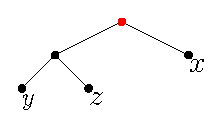
\includegraphics[width=0.2\linewidth]{../figures/vtree.eps}
	\caption{A vTree respected by the formula $(x\land(y\lor z)) \lor (z {
	\color{red}\land } \overline x)$. A conjunction and a corresponding node
are depicted in red.}%
	\label{fig:structed}
\end{figure}

\subsection{Hypergraphs and \texorpdfstring{$\beta$}{(beta)}-acyclic formulas}
Hypergraphs are a well-studied generalization of the concept of graphs. Similar
two an undirected graph, a hypergraph is defined as a set of vertices and edges,
where edges are subsets of the vertices. In contrast to typical graphs,
hypergrphs do not restrict the size of these subsets to two. Hence, each edge
can span no vertex, one vertex or arbitrary many vertices. Most definitions over
graphs such as paths, cycles and connectivity can be extended intuitively for
hypergraphs. However, cyclicity in hypergraphs can be interpreted in different
ways. Here we are interested in $\beta$-acyclic graphs. 

More formally, a hypergraph $H$ is a set of vertices $V$ and a family of subsets
over the vertices, we call them edges $E$. A walk in a hypergraph is a sequence
of alternating vertices and edges that starts and ends with edges, such that
each vertex is a common element for both edges preceding and following this
vertex $(e_1, x_1, \dots, x_n, e_{n+1})$. We call a walk that never visits the
same edge nor the same vertex twice a path. An example of a hyper graph is
depicted in the figure below. [todo]

In order to define $\beta$-acyclic graphs we need to define a
$\beta$-elimination of a graph. Let $\rho := v_1, \dots, v_n$ be an enumeration
of the vertices in the graph. We call $\rho$ a $\beta$-elimination, if for any
two edge $e_1, e_2 \in E$ and $v_i \in e_1 \cap e_2$, holds $e_{1|\geq i}
\subseteq e_2$ or $e_{2|\geq i} \subseteq e_1$, where $e_{\geq i} := \{v_j \in e:
j \geq i\}$. A hypergrph $H$ is $\beta$-acyclic if it admits a
$\beta$-elimination $\rho$.

The hypergraph of a CNF-formula is the hypergraph defined over its variables,
where each clause corresponds to an edge in the graph. More formally, given a
CNF-formula $\varphi$, let $\mathcal{C} := \{C_1, \dots C_m\}$ be the set of all
clauses in this formula. We define the hypergraph $H = (V, E)$ as the
hypergrpah of this formula, where $V := \operatorname{Var}(\varphi)$ and $E :=
\{\operatorname{Var}(C): C \in \mathcal{C}\}$. Note that the same edge might
correspond to multiple clauses with identical variable sets and different
(negated) literals. A Boolean formula $\varphi$ is $\beta$-acyclic if its
hypergraph is.


\subsection{Branch decomposition and MIM-width of a formula}
Back to typical graphs, we define a branch decomposition $T$ of a graph $G = (V,
E)$ as a binary rooted tree $T$, whose leaves are in one-to-one correspondence
with $V$. The maximal-induced-matching width (MIM-width) of a node $t$ in $T$ is
the size of the largest induced matching $M$ of $G[V\setminus V_t, V_t]$. As an
example see the figure below. [todo] The MIM-width of a branch decomposition $T$
$(\operatorname{mimw}(T))$ is the maximum MIM-width of its nodes
$$\operatorname{mimw}(T) = \max\{\operatorname{mimw}(t):t\in V(T)\}.$$ The
MIM-width of a graph $G$ is the minimum MIM-width of a branch decomposition of
this graph.

We define the incidence graph of a CNF-formula as the bipartite graph $G :=(A,
B, E)$, where $A$ is the set of variables of the formula, $B$ the set of the
clauses and a variable is adjacent to a clause if and only if there is a literal
in this clause that corresponds to this variable $$\{x, C\} \in E \iff x \in
\operatorname{Var}(C).$$ The MIM-width of a CNF-formula is the MIM-with of its
incidence graph.


\section{DPLL and solving \#SAT efficiently}
We start this section with a couple of lemmas targeting $\beta$-acyclic graphs.
We aim to gather some useful properties of this class of graphs that we will
exploit in our efficient algorithm afterwards. We begin with the statement of
the main theorem of this part targeting $\beta$-acyclic graphs. After that we
introduce a couple of lemmas that help to prove this theorem. Along this
section, we assume $H$ is an arbitrary $\beta$-acyclic graph. We define an
ordering over the edges of a $\beta$-acyclic graph derived from the
$\beta$-elimination, where for two edges $e, f$, we have $e < f$ if and only if
$\max\{e \Delta f\} \in f$, where $\Delta$ is the symmetric difference of two
sets. This means the ordering is defined by the greatest order of a vertex
appearing in one of the edges but not in the other. Now we denote by $H_e^x$ the
subgraph of $H$ containing all edges reachable form $e$ within a walk having
edges not greater than $e$ upon the previously defined ordering and vertices not
greater than $x$. Note that the edges themselves might contain vertices greater
than $x$. However, such vertices are only not allowed to be walk vertices.
Mathematically speaking $f \in H_e^x$ if and only if there exits a walk $(e_1,
x_1, \dots, x_l, e_{l+1})$, where $e_1 = e$, $e_{l+1} = f$, and $e_{i+1} < e$
and $x_i \leq x$ for all $i \in [l]$. For an example see the figure below
[todo]. We denote the vertex set of a subgraph $H'$ of $H$ by $V(H')$ and the
set of edges by $E(H')$. Moreover, to ease the notation, we use the symbol of a
hypergraph to denote its set of edges, considering the hypergraph as a family of
subsets of vertices. Hence, we write $e\in H$ to denote $e \in V(H)$.


\begin{theorem}\label{theo:hyper}
	$V(H_e^x) \cap V_{\geq x} \subseteq e$ for any $x \in V$ and $e \in E$.
\end{theorem}
In order to prove this theorem we provide the following auxiliary lemmas.
\begin{lemma}
	Let $x, y \in V$ arbitrary and $e, f \in E$, if $V(H_e^x) \cap V(H_f^y)
	\cap V_{\leq x} \neq \emptyset$, then $H_e^x  \subseteq H_f^y$.

	In particular, for all $y \in V(H)$, if $e \in H_f^y$, then $H_e^y
	\subseteq H_f^y$.
\end{lemma}
\begin{proof}[Proof sketch.]
	Choose $g \in H_e^x$ arbitrarily. Per definition, there is a path from
	$e$ to $g$ using edges at most $e$ and vertices at most $x$. Now choose
	$z \in V(H_e^x) \cap V(H_f^y) \cap V_{\leq x}$ arbitrarily. Since $z \in
	V(H_e^x)$ there is similar walk in $H$ from $e$ that ends in $z$. There
	is also a walk in $H$ from $f$ to $z$ using edges at most $f$ and
	vertices at most $y$. by concatenating these three paths we get a walk
	in $H$ from $f$ to $g$. Since $e \leq f$ and $x \leq y$, the resulting
	walk visits edges at most $f$ and vertices at most $y$. 
\end{proof}

\begin{lemma}
	Let $e, f \in H$ two arbitrary edges such that $e < f$. If there exists a vertex $x \in V(H)$, such
	that $x \in e \cap f$, then $e \cap V_{\geq x} \subseteq f$.
\end{lemma}
\begin{proof}[Proof sketch.]
	Directly from the definition of a $\beta$-elimination and that $e < f$.
\end{proof}

We call a path \textbf{decreasing}, if $e_i > e_{i+1}$ for $i \in [l]$ and $x_i
> x_{i+1}$ for all $i\in [l-1]$.
\begin{lemma}\label{lem:decreasing}
	Let $x \in V(H)$, $e \in H$ and $f \in H_e^x$. There exists a decreasing
	path from $e$ to $f$ going through vertices smaller than $x$.
\end{lemma}
\begin{proof}[Proof sketch.]
	There is a walk from $e$ to $f$ in $H$ going through edges at most $e$
	and vertices at most $x$ by the definition of $H_e^x$. It can be shown
	with contradiction, that a shortest path from $e$ to $f$ is decreasing.
	Note that the existence of a walk implies the existence of a path since
	we can "cut" the parts of the walk between two repetitions.
\end{proof}

Now we are ready to prove Theorem~\ref{theo:hyper}.
\begin{proof}[Proof sketch(Theorem~\ref{theo:hyper})]
	By induction over the length of a decreasing path, prove that for any
	edge $f$ on a decreasing path from $e$, it holds that $f \cap V_{\geq x}
	\subseteq e$. Using Lemma~\ref{lem:decreasing}, any edge in $H_e^x$ can
	be reached by a decreasing path and proof is complete.
\end{proof}
An example for the Theorem can be seen in the Figure [todo] below. Intuitively,
this theorem shows the dependence between subgraphs $H_e^x$ for different values
of $e$ and $x$. Hence, for a dynamic programming solution on such subgraphs for
a given problem, we should approach subgraphs with increasing values of $e$ and
$x$.

Now we introduce some more notation in order to provide the main algorithm of
this section. Let $F$ be a given $\beta$-acylic CNF-formula with its hypergraph
$H$. Let $v_1, \dots, v_n$ be a $\beta$-elimination of $H$. Let $F_e^x$ be the
subformula of $F$ corresponding to $H_e^x$ for a vertex $x$ and an edge $e$ in
$H$, i.e. all clauses of $F$ that correspond to edges in $H_e^x$. Mathematically
speaking, $C \in F_e^x \iff \operatorname{Var}(C) \in H_e^x$. For a clause $C$
we define the partial assignment $\tau_C$ over the variables of $C$ as the only
partial assignment that does not satisfy $C$. We define $\tau_C^x :=
\tau_{C|\geq x}$, which means $F_e^x[\tau_C^x]$ for $e := \operatorname{C}$
results from $F_e^x$ by removing variables greater than $x$.

\begin{lemma}
	Let $x \neq x_1 \in \operatorname{Var}(F)$ and let $y$ be the
	predecessor of $x$. Let $e \in H$ be arbitrary and $\tau:(e\cap V_{\geq
	x}) \rightarrow \{\mathbb{0}, \mathbb{1}\}$. Then either $F_e^x[\tau]
	\equiv 1$ or there exists $U \subseteq H_e^x$ such that
	$$F_e^x[\tau] \equiv \bigwedge\limits_{g \in U} F_g^y \left[
	\tau^y_{C_g} \right],$$
	where $C_g$ is an arbitrary clause in $F_e^x$ such that
	$\operatorname{Var}(C_g) = g$. Moreover, all and-gates are decomposable
	and $U$ can be computed in polynomial time.
\end{lemma}
\begin{proof}[Proof sktech.]
	Let $A$ be the set of all edges $g$, such that $\tau \not \models C_g$
	for any corresponding $C_g$. Each clause $C$ such that
	$\operatorname{Var}(C) \notin A$ is satisfied by $\tau$. Choose $U$ as
	the set of "maximal" edges $g \in A$, such that for any edge $f \in A$
	there is an edge $g \in U$ such that $f \in H_g^y$ and no edge in $U$ is
	in the subgraph of any other edge, i.e. for all $f\in U$, $f \notin
	H_g^y$ for all $g$ in $A$. $U$ can be computed by brute-force testing
	all edges and building all subgraphs in polynomial time. The edges in
	$U$ are pairwise disjoint, since we have chosen a maximal set. Hence,
	the and-gate is decomposable.
\end{proof}

\begin{corollary}
	Let $x \neq x_1 \in \operatorname{Var}(F)$ and let $y$ be the
	predecessor of $x$. For every $C \in F$ there exists $U_0, U_1
	\subseteq H_{\operatorname{Var}(C)}^x$ such that 
	$$F_{\operatorname{Var}(C)}^x[\tau_C^x] \equiv (x \land
	\bigwedge\limits_{g \in U_1}F_g^y[\tau_{C_g}^y]) \lor (\lnot x \land
	\bigwedge\limits_{g \in U_2}F_g^y[\tau_{C_g}^y]).$$
	Moreover, all conjunctions are decomposable and $U_0$, $U_1$ can be
	computed in polynomial time.
\end{corollary}
\begin{proof}[Proof sktech.]
	Let $\tau_1 := \tau_C^x \cup \{x \rightarrow \mathbb{1}\}$
	and $\tau_2 := \tau_C^x \cup \{x \rightarrow \mathbb{0})\}$a.
	$$F_{\operatorname{Var}(C)}^x[\tau_C^x] = 
	(x \land F_{\operatorname{Var}(C)}^x[\tau_1])\lor
	(\lnot x \land F_{\operatorname{Var}(C)}^x[\tau_0]).$$
	Apply the previous lemma on each of the terms.
\end{proof}

Now we move to the main theorem of the section describing an algorithm to
compute equivalent dec-DNNF of linear size with linear fanin for a given
$\beta$-acyclic formula. This allows us to solve \#SAT in polynomial time as we
shall see later.

\begin{theorem}
	Let $F$ be a $\beta$-acyclic CNF-formula. One can construct in
	polynomial time in size(F) a dec-DNNF $D$ of size O(size(F)) and fanin
	at most $|H|$ computing $F$.
\end{theorem}
\begin{proof}[Proof sktech.] [todo]
\end{proof}

[todo] {\color{red} concolude this part with the algorithm}

\section{Structured d-DNNF - Lower-bounds for the general approach}
In this subsection we list a couple of results that combined yield a
super-polynomial loewr bound on the size of a structured equivalent d-DNNF. The
paper reference two of the results from other papers (see references) and uses
them to complete the proof.

\begin{theorem}\cite{}[todo]
	There exists an infinite family of $\beta$-acyclic hypergraphs of
	incidence MIM-width $\Omega(n)$ where $n$ is the number of vertices of
	the grpah.
\end{theorem}

Now we introduce the concept of $(Y,Z)$-triangle.
Given a boolean function $r$ over $X$ and let $(Y, Z)$ be a partition of $X$. We
call $r$ a $(Y, Z)$-rectangle, if and only if for every $\tau, \tau' \in \{0,
1\}^X$ such that $\tau \models r$ and $\tau' \models r$ we have $(\tau|Y \cup
\tau'|Z) \models r$.
We call a set $R := \{ r_1, \dots, r_q \}$ a $(Y,Z)$-rectangle cover of a Boolean
function $f$, if $\operatorname{sat}(f) = \bigcup_{i=1}^x \operatorname{sat}
(r_i)$.

\begin{theorem}\cite{}[todo]
	Let $D$ be a DNNF on a set of variables $X$ respecting a vTree T. For
	every vertex $t$ of $T$, there exists an $(X_t, X\setminus
	X_t)$-rectangle cover of $D$ of size at most $|D|$, where $X_t =
	\operatorname{Var}(T_t)$.
\end{theorem}

For a CNF-formula $F$, Let $\hat F := \{K \cup \{c_K\}|K\in F\}$, where we add a
new variable $c_K$ to each clause $K$.
\begin{theorem}
	Let $F$ be a monotone formula of incidence MIM-width $k$. Any structured
	DNNF computing $\hat F$ is of size at least $2^{k/2}$.
\end{theorem}
\begin{lemma}
	Let $X = \{x_1, \dots, x_n\}$ and $Y=\{y_1, \dots y_n\}$ be two disjoint
	sets of variables. The number of $(X, Y)$-rectangles needed to cover the
	CNF-formula $F=\bigwedge_{i=1}^k (x_i \lor y_i)$ is at least $2^k$.
\end{lemma}

\begin{theorem}
	There exists an infinite family $\mathcal{F}$ of $\beta$-acyclic
	CNF-formulas such that for every $F\in \mathcal{F}$ having $n$
	variables, there is no structured DNNF of size less than
	$2^{\Omega(\sqrt n)}$ computing $F$.
\end{theorem}
\section{Conclusion}
[todo]{\Huge \color{red} do not forget conclusion!!}

\end{document}

